%%%%%%%%%%%%%%%%%%%%%%%%%%%%%%%%%%%%%%%%%%%%%%%%%
%
%     Chapter 4   
%
%%%%%%%%%%%%%%%%%%%%%%%%%%%%%%%%%%%%%%%%%%%%%%%%

\chapter{Implementation} % (fold)
\label{cha:implementation}

\section{Social Module} % (fold)
\label{sec:social_module}

Social Module is an abstract interface for accessing each social network service. Each social network service should inherit from the abstract class \texttt{SocialModule} and implement two interfaces:
\begin{description}
	\item[\texttt{get()}:] \hfill \\ 
	connect to the social network service, fetch data having timestamps later than last time get() is called, and return a collection of fetched data.
	\item[\texttt{post(posts)}:] \hfill \\
	 accept a collection of posts, and send them to the social network service.
\end{description}

% section social_module (end)

\section{HUB} % (fold)
\label{sec:hub}

\begin{figure}[htbp]
	\centering
		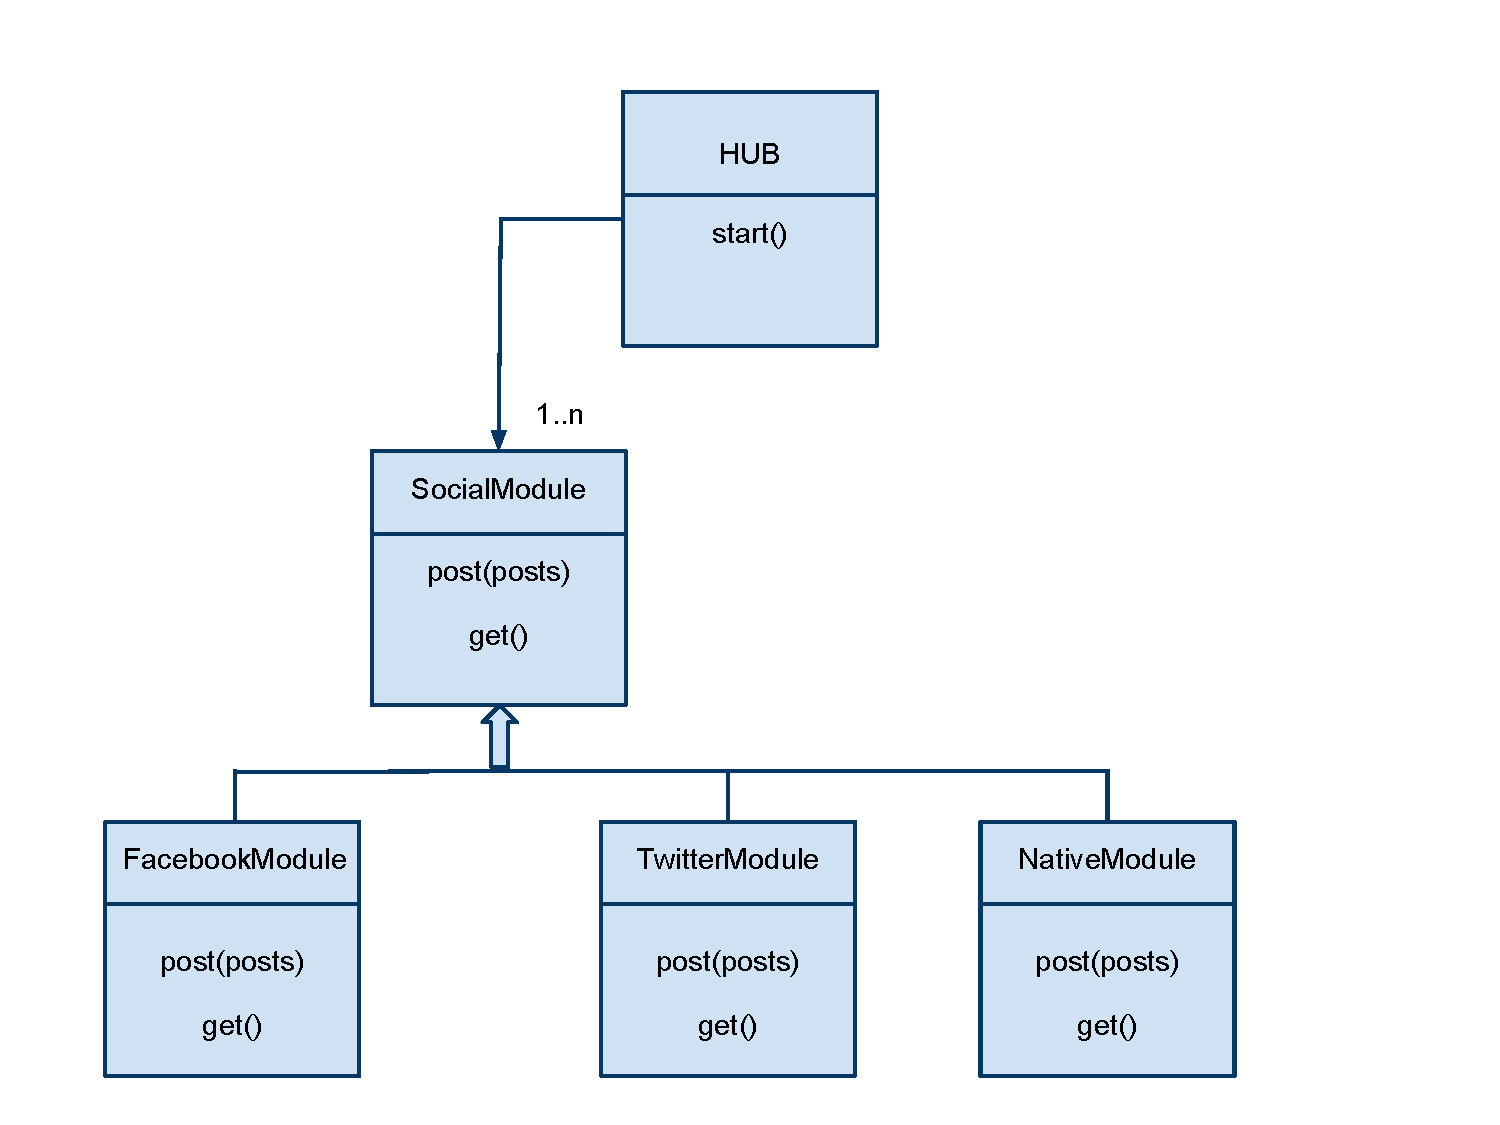
\includegraphics[width = 0.8 \textwidth]{files/graphics/ClassDiagrams.pdf}
	\caption{caption}
	\label{fig:graphics_ClassDiagrams}
\end{figure}

HUB is a component that connects all the social network services and synchronizes them. Essentially, it periodically calls the \texttt{get()} method on each SocialModule. Upon receiving the collections of new posts form all social modules, it synchronizes them to other the social modules. For example, assume that there are three social modules: \texttt{FacabookModule}, \texttt{TwitterModule}, and \texttt{NativeModule}. Once the HUB has received all the new posts from all three modules, it will:
\begin{enumerate}
	\item Push new posts from \texttt{FacebookModule} to \texttt{TwitterModule} and \texttt{NativeModule}
	\item Push new posts from \texttt{TwitterModule} to \texttt{FacebookModule} and \texttt{NativeModule}
	\item Push new posts from \texttt{NativeModule} to \texttt{TwitterModule} and \texttt{FacebookModule}
\end{enumerate}

HUB ensures that data are synchronized between all the social modules.

% section hub (end)

\section{Facebook Module} % (fold)
\label{sec:facebook_module}

Facebook Module's implementation requires a third party library called \emph{Koala}. \emph{Koala} is lightweight Facebook library for Ruby supporting the Graph API. It wraps the entire Facebook Graph API in an class called \texttt{Koala::Facebook::GraphAPI}. Using \emph{Koala} facilitates the object-oriented design of our system.

\subsubsection{OAuth Authentication} % (fold)
\label{ssub:oauth_authentication}

To interact with Social Needle through Facebook, users need to authorize Social Needle to access their Facebook data. Facebook uses OAuth 2.0 Protocol for authentication and authorization. OAuth is an open standard that allows user to share their private data on stored on one site with another without having to give out their user names and passwords. Facebook's JavaScript SDK provides a function to make OAuth authorization easy: \texttt{fb:login-button}. Calling this function in the HTML web page pops up a Facebook dialog for user to authorize Social Needle with certain permissions. For user, we require one permission: 
\begin{description}
	\item[publish\_stream]: \hfill \\
	enabling our application to post content, comments, and likes to a user's stream.
\end{description}
 For administrator, we require an additional permission: 
\begin{description}
	\item[manage\_streams]: \hfill \\
	enabling our application to manage pages the user administrates. 
\end{description} Upon success, the authentication function returns a cookie containing an \texttt{access\_token} with which we can read and write user's data on Facebook.

% subsubsection oauth_authentication (end)

\subsubsection{\texttt{get()} method} % (fold)
\label{ssub:get()_method}

Calling \texttt{get()} method on \texttt{FacebookModule} returns a collection of posts and comments. Internally, \texttt{get()} first sends out a HTTP GET request through Koala to get new posts and comments since last time \texttt{get()} is called (\texttt{FacebookModule} has an attribute \texttt{last\_time} recording that time). This returns a JSON containing the posts with their ids and contents and comments ids related to the posts. Then for each posts that have new comments, it send a HTTP GET request through Koala to get the content of that comment. 
Thus if there are $n$ new posts and $m$ new comments, \texttt{get()} will send out $m+1$ HTTP GET requests.

When \texttt{FacebookModule} is called for the first time, it returns all the posts and comments of that Page since no \texttt{last\_time} is ever recorded. Successive calls only return new posts and comments.

% subsubsection get()_method (end)

\subsubsection{\texttt{post()} method} % (fold)
\label{ssub:post()_method}

\texttt{post()} method accepts a collection of posts and comments. For each post or comment, it is published on the Facebook Page's wall by sending a HTTP POST request through Koala. If the post or comment author has authorized our application to post on his/her stream, we will post using his/her account. Otherwise, we will post using the Page administrator's account.  

% subsubsection post()_method (end)

% section facebook_module (end)

% chapter implementation (end)